\documentclass{article}

\usepackage[utf8]{inputenc}
\usepackage{geometry}
\usepackage{graphicx}
\usepackage{titling}
\usepackage{fancyhdr}
\usepackage{cmbright}
\usepackage{caption}
\usepackage{subcaption}

\geometry{
	a4paper,
	total={170mm, 257mm},
	left=20mm,
	top=20mm
}


\title{Chapter 9: Shapes}
\author{Fharook Shaik}
\date{13 January 2025}

\fancypagestyle{fancy}{
	\fancyhf{}
	\fancyfoot[R]{
\includegraphics[width=3cm]{images/BTULogo_englisch_grau_2x.png}}
	\fancyfoot[L]{\thedate}
	\fancyhead[L]{13869 - Braitenberg Vehicle Praktium}
	\fancyhead[R]{\theauthor}
}

\pagestyle{fancy}

\makeatletter
\renewcommand{\maketitle}{
	\thispagestyle{fancy}
	\null
	\vskip 1em
	\begin{center}
		{\LARGE \@title \par}
	\end{center}
	\vskip 3em
}
\makeatother


\begin{document}

	\maketitle

	\noindent\begin{tabular}{@{}ll}
		Student & \theauthor\\
		Professor &  Dr. Cunningham, Douglas\\
		Matrikel-Nr.: & 5014962
		 
	\end{tabular}

	\section*{Summary}

	In Chapter 9, the focus shifts to how vehicles can perceive and interpret the shapes of objects in their environment. Building on the advancements of Vehicle 8, Vehicle 9 is equipped with systems to detect and analyze shapes, including bilateral symmetry, radial symmetry, and periodic patterns. These enhancements allow the vehicle to interact with its surroundings in more nuanced ways, extending its capacity to understand and respond to the world visually.  
    
	\subsection*{Shape Detection and Bilateral Symmetry}

	The chapter begins by addressing how vehicles can detect shapes independently of color or other irrelevant details. Using lateral inhibition, a process introduced earlier, Vehicle 9 identifies sharp boundaries in its visual field, producing outline drawings of objects. This focus on edges allows the vehicle to analyze shapes as a draftsman would, isolating their external form.  

	The first property of shape explored is \textbf{bilateral symmetry}, which is easy to detect and highly valuable. Vehicle 9 uses a grid of threshold devices, split into two halves: one representing the left side of its visual field and the other the right. Pairs of devices in symmetrical positions are connected by wires that enhance their activity when both receive input. When the vehicle faces a bilaterally symmetrical shape, such as another vehicle, the corresponding threshold devices activate strongly, allowing it to recognize the symmetry.  

	This detector has practical implications. For instance, when a vehicle sees another vehicle heading directly toward it, whether inquisitively, aggressively, or otherwise, the symmetry detector can trigger an appropriate response. This capacity to recognize "another vehicle having me in mind" adds a layer of social awareness, introducing the concept of \textbf{confrontation}—the interaction between two vehicles focusing on each other.

	\begin{figure}[h]
		\centering
		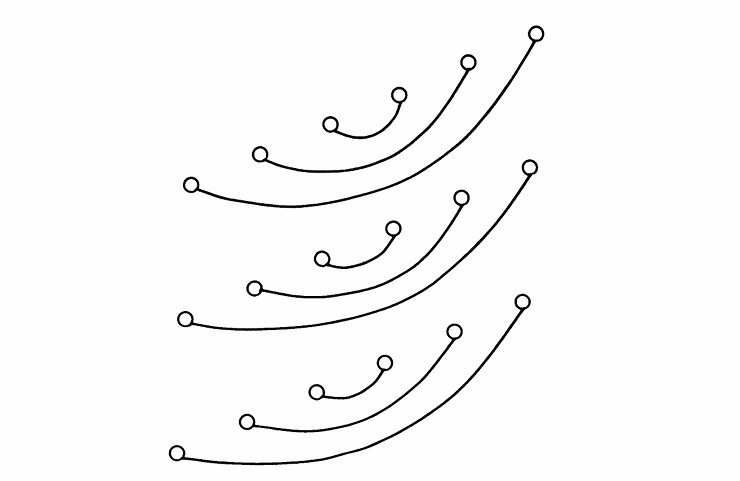
\includegraphics[scale=0.5]{images/figure_16.png}
		\caption{A detector for bilateral symmetry}
		\label{fig:vehicle-16}
	\end{figure}

	Beyond bilateral symmetry, Vehicle 9 is equipped to detect \textbf{radial symmetry}, a feature common in singularities like sources that emit signals or materials in all directions. For example, radial symmetry detectors might identify flowers or patterns that remain unchanged regardless of the angle of observation. This ability is particularly relevant in environments where radial symmetry indicates points of interest, such as energy sources or other vehicles.  

	The chapter also highlights \textbf{periodicity} as a fundamental aspect of form. Periodic patterns may signify collections of identical objects, tracks left by vehicles, or oscillatory movements indicating stored energy. To detect periodicity, Vehicle 9 uses techniques like cross-correlation, comparing its sensory input to periodic templates. Another method involves lateral inhibition, which naturally enhances periodic patterns by emphasizing contrasts at regular intervals. These tools allow the vehicle to identify repetitive structures in its environment, regardless of orientation.
	
	Shape detection has broader implications for interactions between vehicles. Bilateral symmetry, for example, often signifies another vehicle or a potential partner in interaction. In nature, bilateral symmetry plays a role in signaling relationships, as seen in orchids mimicking the shapes of insects to attract pollinators. Similarly, radial symmetry and periodicity help vehicles identify meaningful features in their surroundings, whether sources of energy or patterns left by other vehicles.  

	The chapter emphasizes that the detectors for symmetry and periodicity provide vehicles with inborn concepts that guide their behavior. These detectors are simple in design but powerful in function, allowing vehicles to navigate complex environments with a sense of awareness and intentionality.

	

	\subsection*{Synthetic Psychology and Philosophical Implications}

	The chapter concludes by revisiting the \textit{law of uphill analysis and downhill synthesis.} It highlights how building simple networks can lead to the discovery of implicit concepts, such as space, movement, object reality, and personal interaction. Vehicle 9's ability to detect shapes and patterns demonstrates how inborn concepts, which challenge psychologists and philosophers when studying humans and animals, can emerge from straightforward synthetic designs.  

	Although the chapter focuses on visual input, it suggests that similar detectors could be applied to other sensory modalities, such as touch, smell, or sound. For example, aural periodicity detectors could analyze sound frequencies, mimicking resonators in human auditory systems. This broader application underscores the versatility of the synthetic approach in exploring sensory perception and behavior. 

	\begin{figure}[h]
		\centering
		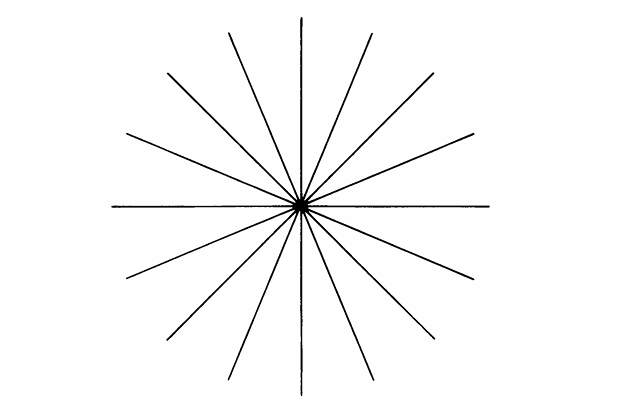
\includegraphics[scale=0.5]{images/figure_17.png}
		\caption{A pattern that is invarian to changes of scale. Vehicle approaching the center of the figure has a constant visual input. Absence of perceived movement may be used as diagnostic for figures with radial symmetry}
		\label{fig:vehicle-17}
	\end{figure}

	Chapter 9 illustrates how Vehicle 9 uses shape detection to enhance its understanding of the environment. By recognizing bilateral and radial symmetry and identifying periodic patterns, the vehicle gains tools to navigate and interact with its surroundings more effectively. These capabilities not only refine the vehicle's perception but also introduce social awareness, enabling it to engage with other vehicles in meaningful ways.  

	Through its exploration of synthetic psychology, the chapter demonstrates how seemingly complex concepts can arise from simple mechanisms, providing new insights into the nature of perception, interaction, and intelligence. Vehicle 9's advancements mark a significant step in bridging the gap between artificial systems and the complexities of real-world behavior.  

\end{document}